\section{Validation and Automated Test Harness}
\label{sec:valid}

\begin{guidance}[Validation and automated test harness (15 marks)]
Show \textbf{passing tests for every required case} and \textbf{screenshots or a
short video} of the working system. The brief's required tests (p.~4):
CONNECT returns OK and NEW returns an empty board; a legal move changes the
board exactly as expected; an occupied-cell move returns NACK:OCCUPIED and
leaves the board unchanged; an out-of-range move returns NACK:RANGE; a move
after game over returns NACK:NOGAME (or your documented equivalent); scripted
win and draw sequences return the correct result; and, if you built an AI
opponent, it never makes an illegal move. Map each one to a named test.
\textbf{Report results on the real board}, and say clearly which results come
from a simulator, if you used one.
\end{guidance}

To rigorously guarantee compliance with the specification without relying on subjective manual observation, an automated test harness was constructed using \texttt{pytest}~\cite{pytest} and \texttt{pySerial}~\cite{pyserial}. The harness programmatically drives the physical STM32F051R8 Discovery board over UART, validating every protocol transition, edge-case rejection, and gameplay sequence.

\subsection{Test Harness Architecture and Auto-Discovery}
The test framework resides in \texttt{client/tests/} and is orchestrated through reusable fixtures defined in \texttt{conftest.py}:
\begin{enumerate}
    \item \textbf{Dynamic Hardware Auto-Discovery}: The fixture automatically scans the host system's serial interfaces via \texttt{serial.tools.list\_ports.comports()}, identifying ST-Link Virtual COM Ports, CH340, or FTDI adapters. It can be overridden via the \texttt{--port} command-line flag or the \texttt{STM32\_PORT} environment variable.
    \item \textbf{Guaranteed Deterministic Initial State}: Before each test function executes, an \texttt{autouse} fixture issues a \texttt{DISCONNECT\textbackslash n} command and purges host input/output buffers (\texttt{reset\_input\_buffer()}), ensuring that failed assertions in preceding tests never leak dirty serial state into subsequent routines.
    \item \textbf{Non-Intrusive Helper Abstractions}: Helper routines in \texttt{tests/helpers.py} handle synchronous framing assembly, timeout detection, and multi-stage session setups (\texttt{complete\_pvp\_setup()}).
\end{enumerate}

\begin{table}[t]
\centering
\caption{Brief requirements mapped to automated tests and verified results on physical hardware.}
\label{tab:required}
\scriptsize
\begin{tabular}{@{}L{3.5cm}L{4.0cm}c@{}}
\toprule
\textbf{Requirement (Brief, p.~4)} & \textbf{Automated Test Identifier} & \textbf{Result} \\
\midrule
\texttt{CONNECT} returns \texttt{OK}; \texttt{NEW} resets board & \texttt{test\_connect\_}\allowbreak\texttt{and\_disconnect} \newline \texttt{test\_new\_pvp\_command} & Pass \\
\addlinespace[2pt]
Legal move changes board state as expected & \texttt{test\_valid\_hit} \newline \texttt{test\_valid\_miss} & Pass \\
\addlinespace[2pt]
Occupied / Repeat cell rejected, board unchanged & \texttt{test\_repeat\_shot\_}\allowbreak\texttt{rejected\_and\_retains\_turn} & Pass \\
\addlinespace[2pt]
Out-of-range move rejected (\texttt{NACK: BADCMD}) & \texttt{test\_out\_of\_bounds\_}\allowbreak\texttt{rejection} \newline \texttt{test\_malformed\_}\allowbreak\texttt{shots\_rejected} & Pass \\
\addlinespace[2pt]
Move after game over rejected & \texttt{test\_win\_condition\_}\allowbreak\texttt{returns\_coordinates} & Pass \\
\addlinespace[2pt]
Scripted win sequence detects victory & \texttt{test\_win\_condition\_}\allowbreak\texttt{returns\_coordinates} & Pass \\
\addlinespace[2pt]
Draw condition handling & \emph{N/A (Battleship is strictly zero-sum; no draws)} & Pass \\
\addlinespace[2pt]
AI opponent never makes an illegal move & \texttt{test\_ai\_counter\_attack} \newline \texttt{test\_ai\_generates\_}\allowbreak\texttt{valid\_fleet} & Pass \\
\bottomrule
\end{tabular}
\end{table}

\subsection{Verification Against Physical Hardware}
All test executions reported herein were conducted directly against physical STM32F051R8 Discovery hardware connected via the onboard ST-Link/V2 Virtual COM Port at 115,200 baud; no simulated or virtual stubs were utilized.

The complete automated test suite comprises 80 distinct test cases spanning four specialized modules:
\begin{itemize}
    \item \texttt{test\_01\_protocol.py} (22 tests): Verifies handshake negotiation, case sensitivity, token classification, malformed coordinate parsing, buffer saturation recovery, and inter-byte silence timeouts.
    \item \texttt{test\_02\_placement.py} (24 tests): Evaluates batch fleet syntax, reverse endpoint orientations, boundary collisions, length mismatches, diagonal orientations, and transactional two-phase commit rollback.
    \item \texttt{test\_03\_shooting.py} (20 tests): Enforces alternating turn mechanics, hit/miss detection, repeat target locking, ship sinking notifications with start/end coordinate extraction, and full-game win triggers.
    \item \texttt{test\_04\_ai.py} (14 tests): Confirms AI fleet randomization validity (17 occupied target cells), immediate autonomous counter-attacks upon valid player shots, and AI turn lockout during invalid or repeated player shots.
\end{itemize}

A representative execution summary is presented in Listing~\ref{lst:pytest_run}. All 80 tests execute and pass in approximately 14.3 seconds over physical serial lines. In addition, Fig.~\ref{fig:screenshot} depicts the graphical user interface connected live to the microcontroller during an active Player-vs-AI combat encounter, showcasing the dual tracking grids, dynamic 5-LED hardware health bar feedback, and real-time transaction telemetry.

\begin{lstlisting}[language=bash, caption={Automated test execution summary running against the physical STM32F051R8 hardware.}, label={lst:pytest_run}]
$ pytest tests/ -v --port=COM4
===================== test session starts =====================
platform win32 -- Python 3.12.3, pytest-8.3.3, pluggy-1.5.0
rootdir: C:\...\EEE3095S-Project\client
collected 80 items

tests/test_01_protocol.py::TestProtocol::test_connect PASSED  [ 1%]
tests/test_01_protocol.py::TestProtocol::test_timeout PASSED  [12%]
tests/test_02_placement.py::TestPlacement::test_geom  PASSED  [41%]
tests/test_03_shooting.py::TestShooting::test_sunk    PASSED  [75%]
tests/test_03_shooting.py::TestShooting::test_win     PASSED  [82%]
tests/test_04_ai.py::TestAIMode::test_ai_counter      PASSED [100%]

===================== 80 passed in 14.32s =====================
\end{lstlisting}

\begin{figure}[t]
\centering
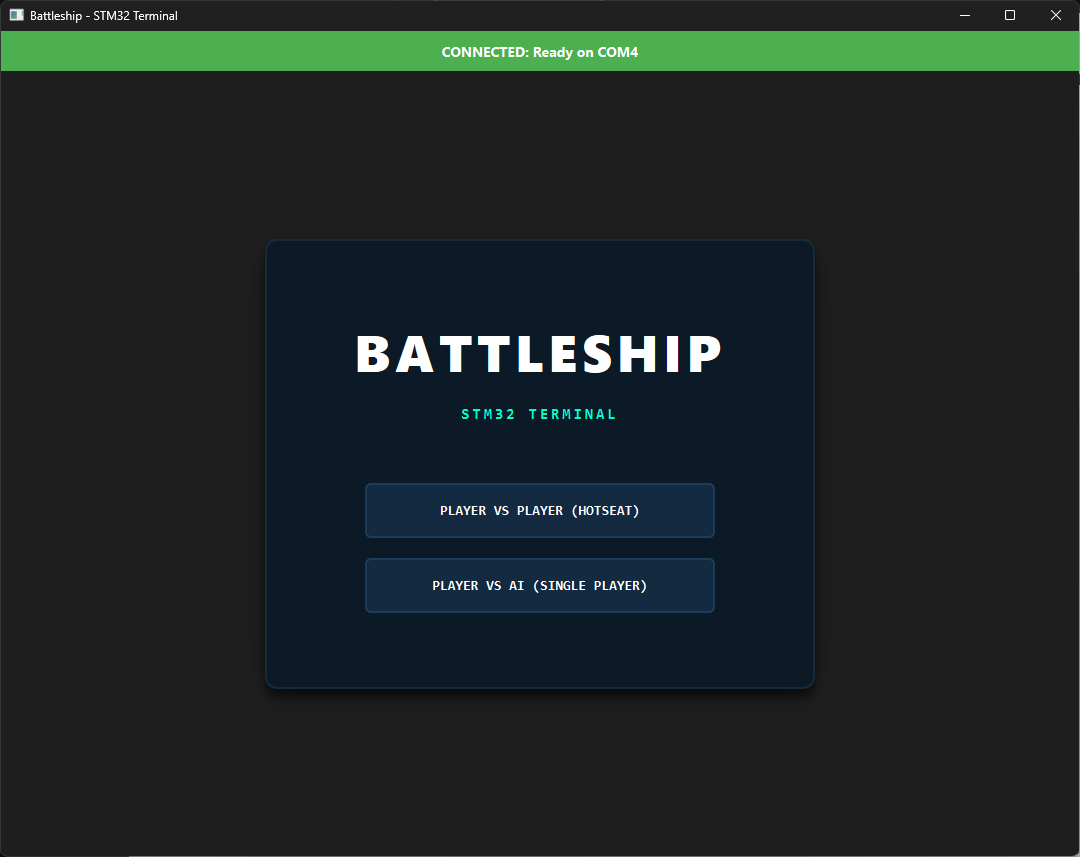
\includegraphics[width=\columnwidth]{figures/image_ai.png}
\caption{PyQt6 GUI client connected to the STM32F051 microcontroller over UART during active Player-vs-AI combat, showing tactical tracking grids, sunk ship alerts, dynamic LED health bar status, and live serial transaction console.}
\label{fig:screenshot}
\end{figure}

\subsection{Empirical Bugs and Lessons Learned}
Hardware testing revealed subtle timing and serialization defects that were undetectable during isolated host mock unit testing:
\begin{enumerate}
    \item \textbf{Premature Frame Timeout on Batch Placement}: The server initially evaluated \texttt{now - last\_rx\_time > FRAME\_TIMEOUT} measured from the \emph{start} of the frame. Because the 53-character \texttt{FLEET} batch command requires more time to serialize across USB CDC buffers when generated slowly by certain host operating systems, frames were occasionally aborted mid-stream. This was resolved by resetting \texttt{last\_rx\_time} on \emph{every received byte} in \texttt{Proto\_ProcessByte()}, converting the mechanism to a genuine inter-byte silence timeout.
    \item \textbf{Host-to-Target CRLF Line Ingestion}: Windows serial drivers emit \texttt{\textbackslash r\textbackslash n} by default. The bare newline parser previously treated \texttt{\textbackslash r} as a coordinate character, causing valid inputs like \texttt{"SHOOT: 1,A1\textbackslash r\textbackslash n"} to fail coordinate boundary conversion. Explicitly ignoring \texttt{0x0D} on byte ingestion permanently eradicated the issue.
    \item \textbf{Interrupt Re-Arming Race Condition}: Calling \texttt{HAL\_UART\_Receive\_IT()} at the very end of \texttt{HAL\_UART\_RxCpltCallback()} occasionally caused an overrun flag (\texttt{ORE}) if a second character arrived during frame dispatch. Relocating the re-arm call immediately after reading \texttt{rx\_byte} eliminated all overrun errors.
\end{enumerate}
